\chapter{Населённые пункты}
\label{ch:human-settlement}

	В главе исследуется объект Викиданных \wdqName{населённый пункт}{486972} и его свойства. В каждом из разделов представлены задачи, решённые с помощью SPARQL-запросов. В их числе: нахождение экземпляров объекта \href{http://www.wikidata.org/entity/Q486972}{населённый пункт}, построение упорядоченного списка стран по суммарному количеству населения, проживающего в \href{http://www.wikidata.org/entity/Q486972}{населённых пунктах}, и списка объектов, сопутствующих \href{http://www.wikidata.org/entity/Q486972}{населённым пунктам} в свойстве \wdProperty{31}{экземпляр}. Также построена диаграмма, показывающая долю населения страны, проживающего в \href{http://www.wikidata.org/entity/Q486972}{населённых пунктах}. Диаграмма показывает, что высокий процент населения, проживающего в \href{http://www.wikidata.org/entity/Q486972}{населённых пунктах}, приходится на менее промышленные страны, в то время как в более индустриальных странах меньшая доля населения проживает в \href{http://www.wikidata.org/entity/Q486972}{населённых пунктах}. 

На 2017 год Википедия описывает примерно половину населённых пунктов (75 тыс.), Викиданные содержат менее 3\% таких поселений (4 тыс.) относительно данных переписи за 2010 год (155,5 тыс.). 

На 2021 год Википедия описывает населённых пунктов , Викиданные содержат менее  таких поселений относительно данных переписи за 2010 год (155,5 тыс.). 

Для улучшения результатов решения вышеописанных задач находили более общие классы и указывали их в исследуемом объекте с помощью свойства \href{http://www.wikidata.org/entity/P31}{экземпляры}. Трудность исследования вызвана отсутствием чёткой типологии населённых пунктов (например, от численности населения) в законодательстве России и в Викиданных.


%%%%
\section{Экземпляры объекта <<Населённый пункт>>}

Для построения списка всех населённых пунктов нам потребуются объект 
\href{http://www.wikidata.org/entity/Q486972}{населённый пункт} и свойство \href{http://www.wikidata.org/entity/P31}{экземпляры}
(листинг ~\protect\ref{lst:human-settlement1}).

\begin{lstlisting}[ language=SPARQL, 
                    caption={\href{https://w.wiki/49WB}{Список всех Населённых пунктов}\protect\footnotemark},
                    label=lst:human-settlement1,
                    texcl 
                    ]
# List of all human settlements
SELECT ?hum ?humLabel 
WHERE 
{
  ?hum wdt:P31 wd:Q486972. # instance of human settlement  
  SERVICE wikibase:label{bd:serviceParam wikibase:language "ru,en"}
}
\end{lstlisting}%
\footnotetext{Получено \num{411393} записи в 2017 году.  Ссылка на SPARQL-запрос: \href{https://w.wiki/49WB}{https://w.wiki/49WB}}

В 2021 году список населённых пунктов получить невозможно из-за большого числа объектов и поэтому слишком долгой работы скрипта. Для получения результата произведем подсчёт всех населённых пунктов (листинг ~\protect\ref{lst:human-settlement2}).

\begin{lstlisting}[ language=SPARQL, 
                    caption={\href{https://w.wiki/49WC}{Количество всех Населённых пунктов}\protect\footnotemark},
                    label=lst:human-settlement2,
                    texcl 
                    ]
# Number of human settlements
SELECT (COUNT(?hum) AS ?count) 
WHERE {
  ?hum wdt:P31 wd:Q486972. # instance of human settlement  
  SERVICE wikibase:label{bd:serviceParam wikibase:language "ru,en"}
}
\end{lstlisting}%
\footnotetext{Получено \num{563126} записей в 2021 году. Ссылка на SPARQL-запрос: \href{https://w.wiki/49WC}{https://w.wiki/49WC}}

Почти пустыми и малоинформативными населёнными пунктами оказались: \href{http://www.wikidata.org/entity/Q31913786}{Беломорск} (\num{25} свойств), \href{http://www.wikidata.org/entity/Q37958167}{Сегежа} (\num{22} свойства), \href{http://www.wikidata.org/entity/Q33522990}{Янишполе} (\num{20} свойств).

Среди отечественных населённых пунктов в Викиданных больше всего свойств по данным ProWD у \href{http://www.wikidata.org/entity/Q128499}{Ялты} (\num{36} свойств). Лидером по всему миру является \href{http://www.wikidata.org/entity/Q1490}{Токио} (\num{73} свойства). \protect\footnotemark

\footnotetext{По данным ProWD: \href{https://prowd.id/dashboards/f64fc6d3d55d/profile}{https://prowd.id/dashboards/f64fc6d3d55d/profile}}


%%%%
\section{Список стран по суммарному количеству населения}

Построим упорядоченный список стран по суммарному количеству населения, проживающего в <<населённых пунктах>> (листинг ~\protect\ref{lst:human-settlement3}).

\begin{lstlisting}[ language=SPARQL, 
                    caption={\href{https://w.wiki/49W2}{Список стран по суммарному количеству населения}\protect\footnotemark},
                    label=lst:human-settlement3,
                    texcl 
                    ]
# List of countries by population in settlements
SELECT ?country ?countryLabel (SUM(?population) as ?sumPopulation)
WHERE
{
  ?hum wdt:P31 wd:Q486972; # instance of human settlement
       wdt:P17 ?country;   # settlement in the ?country
       wdt:P1082 ?population. # settlement has ?population
  
  SERVICE wikibase:label{bd:serviceParam wikibase:language "ru,en"}
}
GROUP BY ?country ?countryLabel 
ORDER BY DESC (?sumPopulation)
\end{lstlisting}%
\footnotetext{Получено \num{161} запись в 2017 году и \num{213} записей в 2021 году. Ссылка на SPARQL-запрос: \href{https://w.wiki/49W2}{https://w.wiki/49W2}}

Для группирования населённых пунктов по странам, используем команду GROUP BY в предпоследней строчке скрипта (листинг ~\protect\ref{lst:human-settlement3}).

Пузырьковая диаграмма на рисунке ~\ref{fig:human-settlement-1} показывает соотношение стран по количеству населения в <<населённых пунктах>>.

\begin{figure}
\centering
	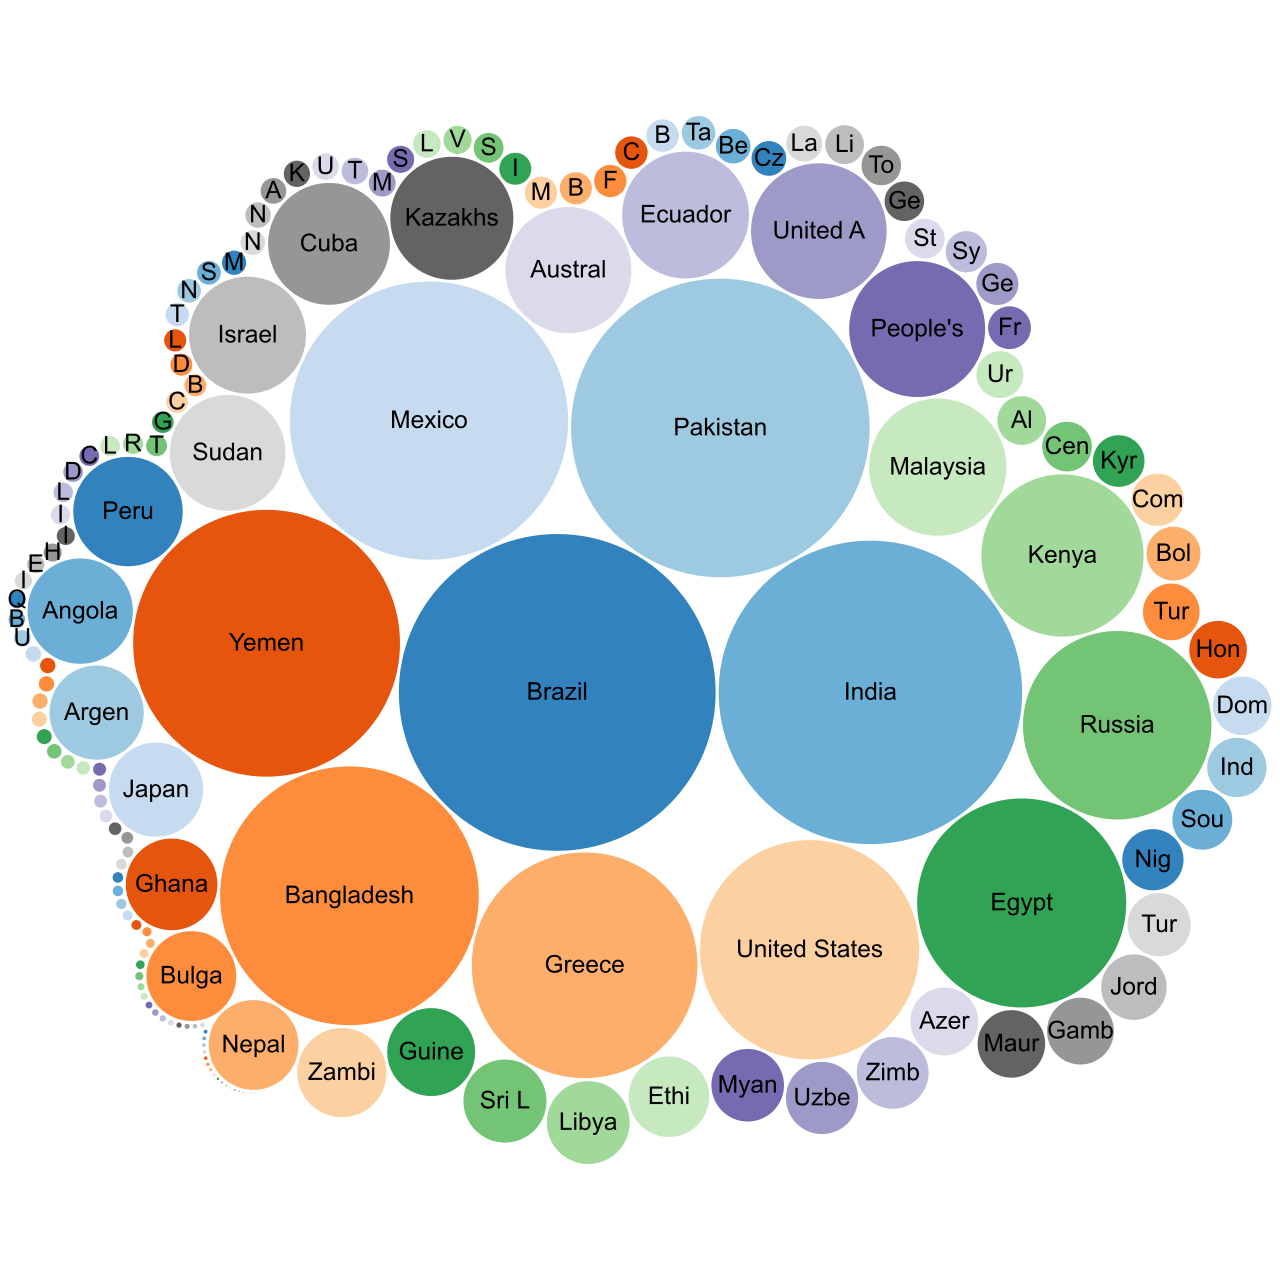
\includegraphics[width=0.9\linewidth]{./chapter/human_settlement/AnnaBubbleHumanSettlement.jpg}
	\label{fig:human-settlement-1}
    \caption[Пузырьковая диаграмма  по суммарному количеству населения в населённых пунктах, 2017.]{Пузырьковая диаграмма  по суммарному количеству населения, проживающего в объектах типа <<населённый пункт>> на 2017 год. Размер пузырька соответствует числу населения для одной страны. Ссылка на SPARQL-запрос: \href{https://w.wiki/49W2}{https://w.wiki/49W2}}
\end{figure}

\begin{figure}
\centering
	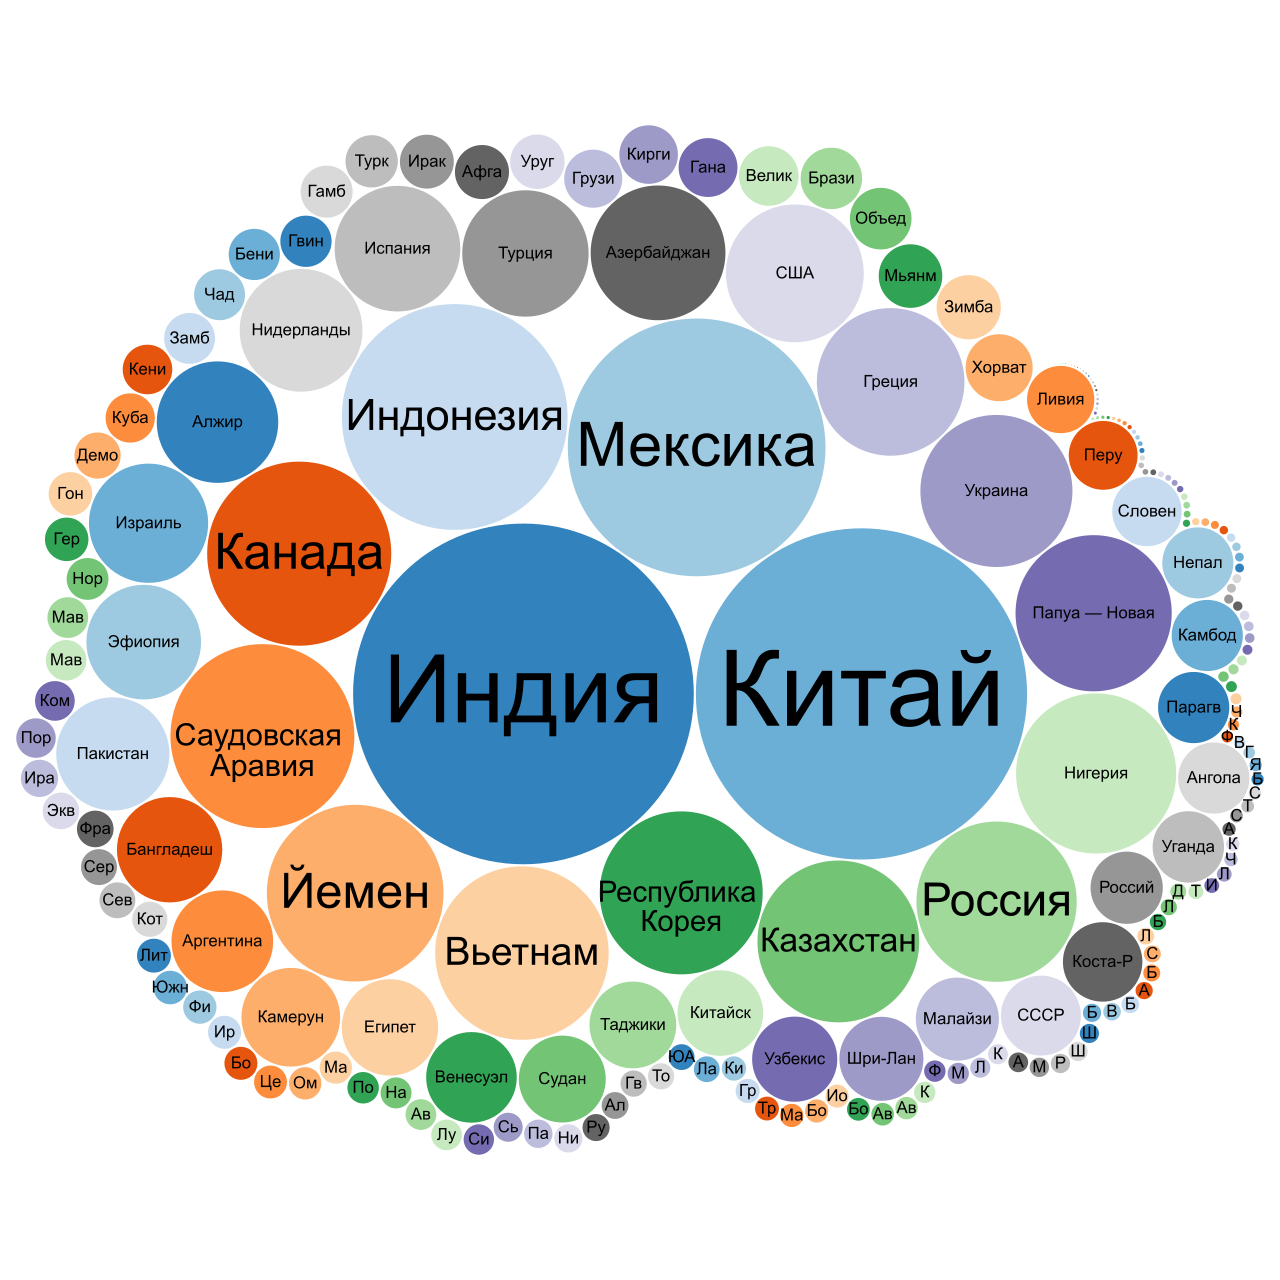
\includegraphics[width=0.9\linewidth]{./chapter/human_settlement/LeonidBubbleHumanSettlement.jpg}
	\label{fig:human-settlement-2}
	\caption[Пузырьковая диаграмма  по суммарному количеству населения в населённых пунктах, 2021.]{Пузырьковая диаграмма  по суммарному количеству населения, проживающего в объектах типа <<населённый пункт>> на 2021 год. Размер пузырька соответствует числу населения для одной страны. Ссылка на SPARQL-запрос: \href{https://w.wiki/49W2}{https://w.wiki/49W2}}
\end{figure}

Итоги запросов в 2017 и 2021 имеют сильно различные результаты. В 2017 году большее количество населения проживало в объектах <<населённый пункт>> в таких странах, как: \href{http://www.wikidata.org/entity/Q155}{Бразилия} (\num{12} млн), \href{http://www.wikidata.org/entity/Q843}{Пакистан} (\num{10} млн), \href{http://www.wikidata.org/entity/Q96}{Мексика} (\num{8} млн), \href{http://www.wikidata.org/entity/Q805}{Йемен} (\num{8} млн), \href{http://www.wikidata.org/entity/Q668}{Индия} (\num{7} млн), \href{http://www.wikidata.org/entity/Q902}{Бангладеш} (\num{7} млн). На рисунке ~\ref{fig:human-settlement-2} можно увидеть, что в 2021 году список первых стран изменился: \href{http://www.wikidata.org/entity/Q668}{Индия} (\num{30} млн), \href{http://www.wikidata.org/entity/Q148}{Китай} (\num{28} млн), \href{http://www.wikidata.org/entity/Q96}{Мексика} (\num{17} млн), \href{http://www.wikidata.org/entity/Q252}{Индонезия} (\num{13} млн), \href{http://www.wikidata.org/entity/Q16}{Канада} (\num{9} млн), \href{http://www.wikidata.org/entity/Q851}{Саудовская Аравия} (\num{9} млн). 
Эти страны имеют пригодные климатические и географические условия для комфортного проживания в относительно небольших населённых пунктах.

%%%%%%%%%%%%%%%%%%%%%%%%%%%%%%%%%%%%%%%%%%%%%%%%%%%%%%%%%%%%%%%%%%%%%%%%%%%%%%%%%%%%%%%%%%%%%%%%%%%%%%%%%%%%%%%%%%%%%%%%%%%%%%%%%%%%%%%%%%%%%%%%%%%%%%%%%%%%%%%%%%%%%%%%%%%%%%%%%%%%%%%%%%%%%%%%%%%%%%%%%%%%%%%%%%%%%%%%%%%%%%%%%%%%%%%%%%%%%%%%%%%%%%%%%%%%
\subsection{Дополнение понятия <<населенный пункт>>}

Попробуем получить более полный результат стрипта (листинг ~\protect\ref{lst:human-settlement3}). Для это нужно изучить \wdqName{населенный пункт}{486972} из свойства \wdProperty{31}{экземпляр}. Если рассмотреть город \wdqName{Петрозаводск}{1895} он имеет четыре класса (\wdqName{административно-территориальная единица России}{192287}; \wdqName{город с населением более \num{100000} человек}{1549591}; \wdqName{населённый пункт}{486972}; \wdqName{город}{7930989}). Трое из этих свойств являются схожими и используются совместно с интересующим нас классом <<населенный пункт>>. Выведем список классов по суммарному упоминанию среди объектов имеющих свойство \wdProperty{1082}{численность населения} в \wdqName{России}{159} (листинг ~\protect\ref{lst:human-settlement4}).

\begin{lstlisting}[ language=SPARQL, 
                    caption={\href{https://w.wiki/4XHP}{Модернизированный список стран по суммарному количеству населения}\protect\footnotemark},
                    label=lst:human-settlement4,
                    texcl 
                    ]
# displaying the number of different classes of a joint human 
# settlements in Russia
SELECT ?klass ?klassLabel (COUNT(?klass) AS ?count) 
  (GROUP_CONCAT(DISTINCT ?humLabel; SEPARATOR = "; ") AS ?countries) 
WHERE {
 {
  SELECT ?klass ?klassLabel ?humLabel WHERE {
   ?hum wdt:P17 wd:Q159.  # settlement in the Russia
   ?hum wdt:P31 wd:Q486972. # settlement has human-settlements
   ?hum wdt:P1082 ?population. # settlement has ?population
   ?hum wdt:P31 ?klass. # settlement has other ?klass
   SERVICE wikibase:labe{bd:serviceParam wikibase:language"ru,en".
     ?klass rdfs:label ?klassLabel.
     ?hum rdfs:label ?humLabel.}
  }
 }
}
GROUP BY ?klass ?klassLabel
ORDER BY DESC (?count)
\end{lstlisting}%
\footnotetext{Как и ожидалось класс <<населенный пункт>> оказался не на первом месте и набрал всего \num{1122} упоминаний. Ссылка на SPARQL-запрос: \href{https://w.wiki/4XHP}{https://w.wiki/4XHP}}

Обратим внимание на следующие классы: \wdqName{сельское поселение в России}{634099}~--- \num{18102}, \wdqName{деревня}{5084}~--- \num{14760}, \wdqName{село}{532}~--- \num{9844}, \wdqName{посёлок}{2514025}~--- \num{4413}, \wdqName{хутор}{2023000}~--- \num{1729},  \wdqName{посёлок городского типа России}{15078955}~--- \num{665}. Попробуем получить еще раз результат скрипта (листинг ~\protect\ref{lst:human-settlement3}) используя новые классы. Это позволит избавится от подсчета городов упоминаемых как <<населенный пункт>> (листинг ~\protect\ref{lst:human-settlement5}).

\begin{lstlisting}[ language=SPARQL, 
                    caption={\href{https://w.wiki/4XHv}{Список классов по суммарному упоминанию среди объектов имеющих свойство численность населения в России}\protect\footnotemark},
                    label=lst:human-settlement5,
                    texcl 
                    ]
# Modernized list of countries by population in settlements
SELECT ?country ?countryLabel (SUM(?population) as ?sumPopulation) 
WHERE{
  VALUES ?type {
        wd:Q634099
        wd:Q5084
        wd:Q532
        wd:Q2514025
        wd:Q2023000
        wd:Q15078955
  }
  ?hum wdt:P31 ?type. # instance of human settlement
  ?hum wdt:P17 ?country.   # settlement in the ?country
  ?hum wdt:P1082 ?population. # settlement has ?population
  SERVICE wikibase:label{bd:serviceParam wikibase:language "ru,en"}
}
GROUP BY ?country ?countryLabel
ORDER BY DESC (?count)
\end{lstlisting}%
\footnotetext{Как и ожидалось Россия оказалась на первом месте и набрала число населения \num{53798270}. На втором месте оказались Нидерланды с результатом \num{11893141}. Открыв от второго места 42 млн Ссылка на SPARQL-запрос: \href{https://w.wiki/4XHv}{https://w.wiki/4XHv}}

Числиность насиления России в результатах скриптов (листинг ~\protect\ref{lst:human-settlement3}) и (листинг ~\protect\ref{lst:human-settlement5}) получилась \num{6494645} и \num{53798270} соответственно. Из чего следует, что нужно произвести уточнение и для других стран.

 Как это сделать пока что не понятно, так как запрос превышает время ожидания и не выдает результатов. А перебирать каждую крупную страну плохой вариант. Возможно позже появится хорошее решиние этой задачи.

%%%%%
\subsection{Полнота Викиданных}

Населённый пункт — это общее название мест с постоянными жителями\footnote {Ожегов С. И. Толковый словарь русского языка, 2003}. По версии редакторов Викиданных в понятие насёленный пункт входят города, сёла, деревни и другие\footnote{Полный список можно увидеть в разделе этой главы «Cписок объектов, сопутствующих "human\_settlement" в "instance of"».}.
Точной информации о количестве населённых пунктов в мире не было найдено. Поэтому проверим полноту населённых пунктов, которые есть в Викиданных и которые использовались для решения задачи. Была поставлена задача: построить упорядоченный список стран по суммарному количеству населения, проживающего в \href{http://www.wikidata.org/entity/Q486972}{населённых пунктах}. Для этого напишем \href{https://w.wiki/4FUz}{SPARQL-запрос} \footnotemark, который выведет населённые пункты с незаполненным свойством \href{http://www.wikidata.org/entity/P1082}{численность населения}. 
\footnotetext{ В 2017 году этот запрос выдал \num{372997} таких населённых пунктов. Произведя расчеты получаем, что только у 9,3\% населенных пунктов мира указано количество населения (свойство \wdProperty{1082}{численность населения}). Проводя ту же проверку в 2021 году, запрос выдал \num{507078} таких населённых пунктов. Получаем 11,2\% населенных пунктов мира с заполненным свойство 'численность населения'. Ссылка на SPARQL-запрос: \href{https://w.wiki/4FUz}{https://w.wiki/4FUz}} 
А теперь посмотрим населённые пункты, у которых не указана принадлежность к какой-либо стране~--- \href{https://w.wiki/4FV8}{SPARQL-запрос}\footnotemark.

\footnotetext{В 2017 году таких нашлось \num{8427} объектов. В 2021 году таких объектов уже существенно больше~--- \num{27824}. Поэтому в результате решения данной задачи получились неполная картина о суммарном количестве населения в населённых пунктах по странам. Ссылка на SPARQL-запрос: \href{https://w.wiki/4FV8}{https://w.wiki/4FV8}}

Рассмотрим населённые пункты России. По данным проекта "Населённые пункты России/Статистика" Русская Википедия содержит приблизительно 75 тыс. статей о населённых пунктах России. По переписи 2010 года в России 155 510 населённых пунктов. Проверим, сколько объектов содержится в Викиданных о населённых пунктах России с помощью следующего \href{https://w.wiki/4FVE}{SPARQL-запроса}\protect\footnotemark. 

\footnotetext{В 2017 году было получено \num{4113} объектов, что составляет 2,6\% от общего числа населённых пунктов по переписи за 2010 год. В 2021 году запрос выдал \num{17425} объектов, что составляет 11,2\% от общего числа населённых пунктов. Таким образом, в Викиданных содержится слишком мало информации о населённых пунктах России. Ссылка на SPARQL-запрос: \href{https://w.wiki/4FVE}{https://w.wiki/4FVE}}

Итак, степень заполненности Викиданных по населённым пунктам низкая. А именно, у некоторых городов, поселков, деревень и других населённых пунктов на Викиданны отсутствует свойство \href{http://www.wikidata.org/entity/Q21503252}{экземпляр}, значением которого может быть \href{http://www.wikidata.org/entity/Q486972}{населённый пункт}. Кроме того, есть почти пустые и плохо проработанные объекты. Для решения этих проблем необходимо заполнять эти свойства и связывать между собой объекты Викиданных.

%%%%%
\section{Доля населения страны, проживающего в human\_settlement}

Построим упорядоченный список стран доли населения (в процентах), проживающего в \href{http://www.wikidata.org/entity/Q486972}{населённых пунктах} относительно числа всех жителей страны (листинг ~\protect\ref{lst:human-settlement5}).

\begin{lstlisting}[ language=SPARQL, 
                    caption={\href{https://w.wiki/4Cza}{соотношение количества людей, проживающих в населённых пунктах, к количеству людей, проживающих в стране}\protect\footnotemark},
                    label=lst:human-settlement5,
                    texcl 
                    ]
# An ordered list of the ratio of the number of people living in 
"settlement" to the number of inhabitants in the country.
SELECT ?countryLabel (SUM(?population / ?pop) 
	as ?proportionPopulation) (?proportionPopulation
	 * 100 as ?percentPopulation)
WHERE {
  ?hum wdt:P31 wd:Q486972.    # instances of human settlement  
  ?hum wdt:P17 ?country.      # country 
  ?hum wdt:P1082 ?population. # population
  ?country wdt:P1082 ?pop.    # population in the country

  SERVICE wikibase:label{bd:serviceParam wikibase:language "ru,en"}
  }
GROUP BY ?country ?countryLabel
ORDER BY DESC (?percentPopulation)
\end{lstlisting}%
\footnotetext{Получено \num{158} записей в 2017 году и \num{206} записей в 2021 году. \href{https://w.wiki/4T4s}{Ссылка.}}

Столбчатая диаграмма на рисунке ~\ref{fig:human-settlement-3} позволяет увидеть для каждой отдельной страны отношение количества людей, проживающих в \href{http://www.wikidata.org/entity/Q486972}{населённых пунктах}, к числу жителей в стране на 2017 год.

\begin{figure*}
    \setlength{\fboxsep}{0pt}%
    \setlength{\fboxrule}{1pt}%
    \fcolorbox{gray}{gray}{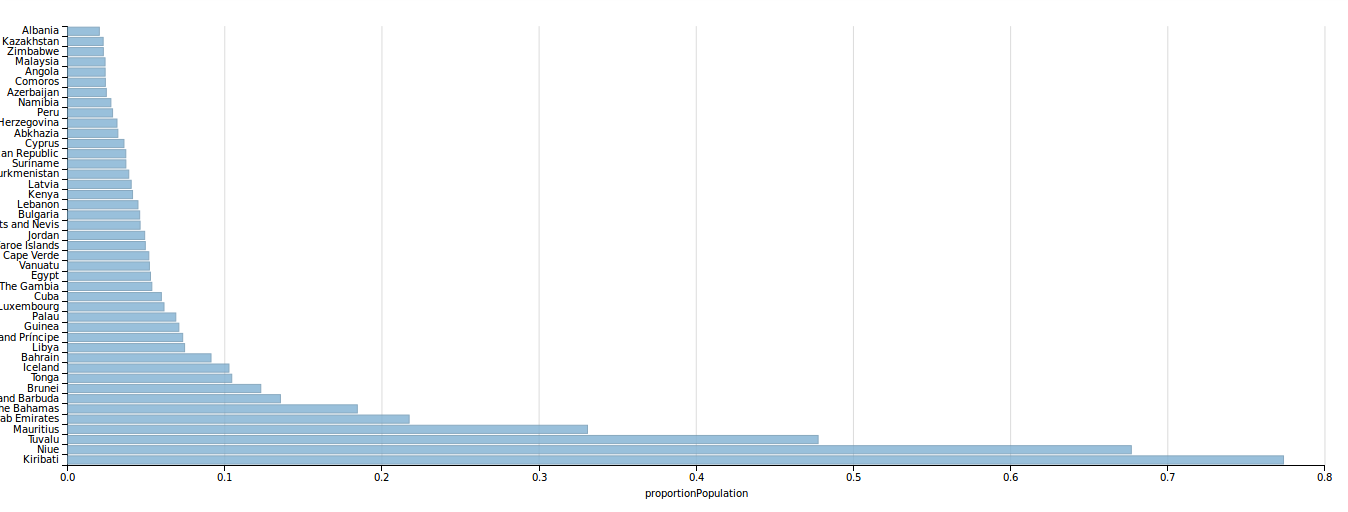
\includegraphics[width=1\linewidth]{./chapter/human_settlement/AnnaShareHumanSettlement.png}}
	\label{fig:human-settlement-3}
	\caption[Диаграмма доли населения страны. Карелия, 2017.]{Диаграмма доли населения страны, проживающего в "населённых пунктах" (2017). Ссылка на SPARQL-запрос: \href{https://w.wiki/4T4s}{https://w.wiki/4T4s}.}%
\end{figure*} 

\begin{figure*}
    \setlength{\fboxsep}{0pt}%
    \setlength{\fboxrule}{1pt}%
    \fcolorbox{gray}{gray}{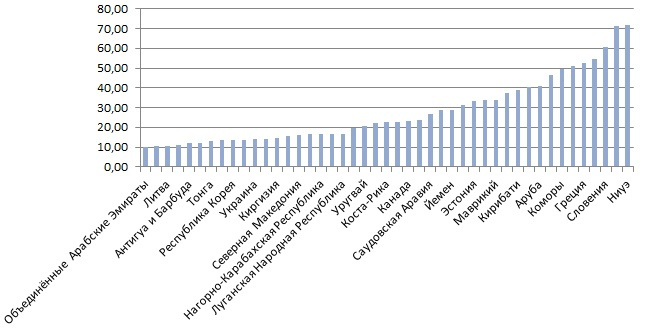
\includegraphics[width=1\linewidth]{./chapter/human_settlement/LeonidShareHumanSettlement.jpg}}
	\label{fig:human-settlement-4}
	\caption[Диаграмма доли населения страны, 2021.]{Диаграмма доли населения страны, проживающего в <<населённых пунктах>> (2021). Ссылка на SPARQL-запрос: \href{https://w.wiki/4T4s}{https://w.wiki/4T4s}}%
\end{figure*} 

На рисунке ~\ref{fig:human-settlement-3} из графика видно, что наиболее высокий процент в 2017 году приходился на следующие страны: Кирибати (78\%), Ниуэ (70\%), Греция (53\%), Тувалу (48\%), Коморы (43\%), Маврикий (42\%). В 2021 году появились изменения : Ниуэ (72\%), Папуа — Новая Гвинея (71\%), Словения (61\%), Фарерские острова (54\%), Греция (53\%), Маршалловы Острова (51\%). Интересно заметить, что в основном это маленькие островные государства. Вероятно, большая часть жителей этих стран сконцентрирована в населённых пунктах.

На 2017 год рассматривая отдельно страны большой восьмёрки, доля жителей в \href{http://www.wikidata.org/entity/Q486972}{населённых пунктах} составила: \href{http://www.wikidata.org/entity/Q159}{Россия} (\num{2.98}\%), \href{http://www.wikidata.org/entity/Q30}{США} (\num{1.76}\%), \href{http://www.wikidata.org/entity/Q17}{Япония} (\num{0.80}\%), \href{http://www.wikidata.org/entity/Q16}{Канада} (\num{0.26}\%), \href{http://www.wikidata.org/entity/Q142}{Франция} (\num{0.20}\%), \href{http://www.wikidata.org/entity/Q183}{Германия} (\num{0.24}\%), \href{http://www.wikidata.org/entity/Q145}{Великобритания} (\num{0.18}\%), \href{http://www.wikidata.org/entity/Q38}{Италия} (\num{0.07}\%). В 2021 году значения заметно снизились: \href{http://www.wikidata.org/entity/Q159}{Россия} (0.045\%), \href{http://www.wikidata.org/entity/Q30}{США} (\num{0.014}\%), \href{http://www.wikidata.org/entity/Q17}{Япония} (\num{0.008}\%), \href{http://www.wikidata.org/entity/Q16}{Канада} (\num{0.23}\%), \href{http://www.wikidata.org/entity/Q142}{Франция} (\num{0.005}\%), \href{http://www.wikidata.org/entity/Q183}{Германия} (\num{0.005}\%), \href{http://www.wikidata.org/entity/Q145}{Великобритания} (\num{0.014}\%), \href{http://www.wikidata.org/entity/Q38}{Италия} (\num{0.0005}\%). Отметим, что это страны промышленно развитые.

Построенная диаграмма подтверждает следующую гипотезу: высокий процент населения страны, проживающего в \wdqName{населённых пунктах}{486972}, указывает на более аграрную страну. В действительности имеется возможность развития сельского хозяйства в этих странах. Исходя из диаграммы и запроса видно, что наиболее высокий процент населения страны, проживающего в населённых пунктах, приходится на островные, южные, жаркие страны, в которых, по-видимому, менее развита промышленность (маленькая территория, небольшое количество населения, удалённость от материков). А индустриальные страны (большой восьмёрки) имеют очень низкий процент населения страны, проживающего в населённых пунктах.

%%%%%
\section{Cписок объектов, сопутствующих human\_settlement в instance of }

Попробуем получить список объектов имеющих свойство населённый пункт. У каждого объекта в Викиданных есть свойство \wdProperty{31}{экземпляр}. Это свойство определяет класс или категорию к которому относится каждый объект в Викиданных. Если рассмотреть город \wdqName{Петрозаводск}{1895} он имеет четыре класса (\wdqName{административно-территориальная единица России}{192287}; \wdqName{город с населением более \num{100000} человек}{1549591}; \wdqName{населённый пункт}{486972}; \wdqName{город}{7930989}). Трое из этих свойств являются схожими. Один из них и есть наш исследуемый объект (населённый пункт).  

Главная трудность вызвана отсутствием чёткой типологии населённых пунктов (например, от численности населения) в законодательстве России и в Викиданных. Поэтому представляет интерес получение списка объектов, сопутствующих объекту населённый пункт в свойстве экземпляр, с помощью следующего скрипта (листинг ~\protect\ref{lst:human-settlement6}).

\begin{lstlisting}[ language=SPARQL, 
                    caption={\href{https://w.wiki/49XL}{Cписок объектов, сопутствующих "human\_settlement" в "instance of"}\protect\footnotemark},
                    label=lst:human-settlement6,
                    texcl 
                    ]
# List of objects accompanying "human\_settlement" in the property
# "instance of"
SELECT ?inst (COUNT(?hum) as ?sumHum) 
WHERE{          
  ?hum wdt:P31 wd:Q486972; # instance of human settlement
         wdt:P31 ?inst.      # other objects in instance

  SERVICE wikibase:label{bd:serviceParam wikibase:language "ru,en"}
}  
GROUP BY ?inst
\end{lstlisting}%
\footnotetext{Получено 610 записей в 2017 году и \num{1245} записей в 2021 году. Ссылка на SPARQL-запрос: \href{https://w.wiki/49XL}{https://w.wiki/49XL}}

Во-первых, выключим из рассмотрения такие населённые пункты, которые имеют в списке экземпляров только населённый пункт. Результат не ухудшится, так как в него не будут включёны экземпляры только типа населённый пункт. С этой целью внесём в наш скрипт строку \num{9} и получим фильтр для отбора нужных поселений.

Во-вторых, в строке \num{8} уберем такие объекты переменной \emph{?inst}, которые имеют свойство \wdqName{государство}{17}. Это позволит отсечь сотни типов населённых пунктов специфичных для отдельных стран, например, административно-территориальная единица России.

Эти ограничения позволили выполнить запрос по всем странам мира за приемлемое время (87 мс) (листинг ~\protect\ref{lst:human-settlement7}).

\lstset{numbers=left, firstnumber=1, frame=single}
\begin{lstlisting}[ language=SPARQL, 
                    caption={\href{https://w.wiki/49XK}{Cписок объектов, сопутствующих "human\_settlement" в "instance of"}\protect\footnotemark},
                    label=lst:human-settlement7,
                    texcl 
                    ]
# Modernized list of objects accompanying "human\_settlement" in 
# the property "instance of"
SELECT ?inst ?instLabel (COUNT(?hum) as ?sumHum) 
WHERE{ 
  ?hum wdt:P31 wd:Q486972;  # instance of human settlement
       wdt:P31 ?inst.       # other objects in instance
  
  MINUS {?inst wdt:P17 []}. # without country
  FILTER(?inst != wd:Q486972 ). # without human settlement
  SERVICE wikibase:label{bd:serviceParam wikibase:language "ru,en"}
}  
GROUP BY ?inst ?instLabel
\end{lstlisting}%
\footnotetext{Получено 355 записей в 2017 году и 707 записей в 2021 году. Ссылка на SPARQL-запрос: \href{https://w.wiki/49XK}{https://w.wiki/49XK}}

На 2017 год в число таких объектов входят:
\begin{enumerate} 
  \item \href{http://www.wikidata.org/entity/Q532}{Cёла (Village)}~--- \num{2844}.
  \item \href{http://www.wikidata.org/entity/Q15284}{Муниципалитеты (municipality)}~--- \num{1181}.
  \item \href{http://www.wikidata.org/entity/Q5084}{Деревни (hamlet)}~--- \num{662}.
  \item \href{http://www.wikidata.org/entity/Q839954}{Археологические памятники (archaeological site)}~--- \num{425}.
  \item \href{http://www.wikidata.org/entity/Q3257686}{Местные поселения (locality)}~--- \num{425}.
\end{enumerate}

На 2021 год в число таких объектов входят:
\begin{enumerate} 
  \item \href{http://www.wikidata.org/entity/Q106505070}{Поселение в доисторические времена (Settlement of prehistoric times)}~--- \num{5021}.
  \item \href{http://www.wikidata.org/entity/Q532}{Cёла (Village)}~--- \num{4853}.
  \item \href{http://www.wikidata.org/entity/Q15303838}{Местоположение муниципалитета (Municipality seat)}~--- \num{3376}.
  \item \href{http://www.wikidata.org/entity/Q106492558}{Поселение в доисторические времена (Settlement of prehistoric times)}~--- \num{2288}.
  \item \href{http://www.wikidata.org/entity/Q106491339}{Поселение неолита (Neolithic settlement)}~--- \num{2095}.
\end{enumerate}

Также в 2021 году было преложеная еще одна модернизация скрипта (листинг ~\protect\ref{lst:human-settlement7}). А именно отсечь доисторические поселения таких типов, как поселения \wdqName{латенского периода}{106505016}, \wdqName{бронзового века}{106491277}каменного века и \wdqName{доисторического времени, где есть письменность}{106505070} поселение в доисторические времена, без явного указания этих трёх объектов. 
Было изучено, что есть общего у объектов <<латенского периода>> и <<каменного века>> и <<доисторического времени, где есть письменность>> на Викиданных. Будем фильтровать объекты, которые являются подклассом такого объекта, который, в свою очередь, является экземпляром объектов \wdqName{археологической культуры}{465299}, \wdqName{исторического периода}{11514315}, \wdqName{археологического века}{15401699}, \wdqName{всемирной истории}{200325} и \wdqName{геологического периода}{392928}. В итоге получился такой скрипт (листинг ~\protect\ref{lst:human-settlement8}).

\lstset{numbers=left, firstnumber=1, frame=single}
\begin{lstlisting}[ language=SPARQL, 
                    caption={\href{https://w.wiki/4YpA}{Cписок объектов, сопутствующих "human\_settlement" в "instance of"}\protect\footnotemark},
                    label=lst:human-settlement8,
                    texcl 
                    ]
# Modernized list of objects accompanying "human\_settlement" in the 
# property "instance of"
SELECT ?inst ?instLabel (COUNT(?hum) as ?sumHum)
WHERE{
  VALUES ?type {
    wd:Q465299   #archaeological culture 
    wd:Q11514315 #historical period
    wd:Q15401699 #archaeological age
    wd:Q200325   #human history
    wd:Q392928   #geological period
  }
  ?hum wdt:P31 wd:Q486972.    # instance of human settlement
  ?hum wdt:P31 ?inst.#other objects in instance of human settlement
  ?inst wdt:P31 ?test.#instance of other objects 
  ?test wdt:P31 ?typ.#instance of instance of other objects 
  MINUS {?inst wdt:P17 []}.   # without country
 # without human settlement and prehistoric settlements
  FILTER(?inst != wd:Q486972 && ?typ != wd:Q465299 
		&& ?typ != wd:Q11514315 && ?typ != wd:Q15401699 
		&& ?typ != wd:Q200325 && ?typ != wd:Q392928 ). 
  SERVICE wikibase:label{bd:serviceParam wikibase:language"ru, en"}
}
GROUP BY ?inst ?instLabel
ORDER BY DESC (?sumHum)
\end{lstlisting}%
\footnotetext{Получено 89 записей. Ссылка на SPARQL-запрос: \href{https://w.wiki/4YpA}{https://w.wiki/4YpA}}

В число таких объектов входят:
\begin{enumerate} 
  \item \href{http://www.wikidata.org/entity/Q5084}{ деревня ()}~--- \num{8820}.
  \item \href{http://www.wikidata.org/entity/Q2514025}{ посёлок ()}~--- \num{1590}.
  \item \href{http://www.wikidata.org/entity/Q2593777}{ могильник ()}~--- \num{1200}.
  \item \href{http://www.wikidata.org/entity/Q814254}{  (feature)}~--- \num{1095}.
  \item \href{http://www.wikidata.org/entity/Q23442}{ остров ()}~--- \num{1085}.
\end{enumerate}

%%%%%
\section{Отечественные учёные на селе и в городе}

Попробуем подсчитать число отечественных учёных, родившихся в сельских и городских типах населённых пунктов. И сравнить эти числа.
Поделим это задание на четыре части:
\begin{enumerate}
  \item Выявить список сельских и список городских типов поселений именно в России.
  \item Выявить способ определения отечественных ученых.
  \item Сделать такую диаграмму на которой разным цветом будут указаны разные научные направления (математики, физики, химики и так далее) для учёных родившихся в селах.
  \item Сделать вторую диаграмму — по городским поселениям и сравнить результаты.
\end{enumerate}

%%%%%
\subsection{Список сельских и список городских типов поселений именно в России}

Список сельских: (ссылка на раздел выше)

\begin{enumerate}
  \item \wdqName{vilage}{532}
  \item \wdqName{ rural settlement of Russia}{634099}
  \item \wdqName{rural settlement}{10354598}
  \item \wdqName{ hamlet}{5084}
  \item \wdqName{posyolok}{2514025}
  \item \wdqName{khutor}{2023000}
  \item \wdqName{urban-type settlement in Russia}{15078955}
\end{enumerate}

Список городских: (ссылка на главу о городах) 
\begin{enumerate}
  \item \wdqName{city(1m+)}{1637706}
  \item \wdqName{city(100k+)}{1549591}
  \item \wdqName{city+town}{7930989}
  \item \wdqName{town}{515}
  \item \wdqName{small town}{3957}
\end{enumerate}
%%%%%
\subsection{Выявить способ определения отечественных ученых}

Список гражданства:
\begin{enumerate}
  \item \wdqName{Russian Empire }{34266}
  \item \wdqName{Russian Republic}{139319}
  \item \wdqName{Soviet Union}{15180}
  \item \wdqName{Russia}{159}
\end{enumerate}

Список академий: (ссылка на вкр + одна моя)
\begin{enumerate}
  \item \wdqName{academy of sciences}{414147}
  \item \wdqName{learned society}{955824}
  \item \wdqName{scientific society}{74801 }
  \item \wdqName{academy}{162633}
  \item \wdqName{research institute}{31855 }
  \item \wdqName{educational institution}{2385804  }
  \item \wdqName{Russian Academy of Science}{83172}
\end{enumerate}
%%%%%
\subsection{Построение диаграммы на которой разным цветом будут указаны разные научные направления для учёных родившихся в селах.}


\lstset{numbers=left, firstnumber=1, frame=single}
\begin{lstlisting}[ language=SPARQL, 
                    caption={\href{https://w.wiki/4YpA}{Cписок объектов, сопутствующих "human\_settlement" в "instance of"}\protect\footnotemark},
                    label=lst:human-settlement9,
                    texcl 
                    ]
# Conclusion of the number of Russian scientists born in 
# the settlement by occupation and year of birth
SELECT ?hum ?_inception ?year ?specLabel ?count ?totalspec WHERE {
  SELECT DISTINCT  (SAMPLE(?year) AS ?year) 
	(COUNT(?humLabel) AS ?count)  
	(GROUP_CONCAT(DISTINCT ?specLabel; SEPARATOR=", ") AS ?totalspec) 
	WHERE {
    VALUES ?state { # types of citizenship
      wd:Q34266   # Russian Empire 
      wd:Q139319  # Russian Republic
      wd:Q15180   # Soviet Union
      wd:Q159     # Russia
    }
    VALUES ?placeb { # types of settlements
      wd:Q532        # vilage
      wd:Q634099     # rural settlement of Russia
      wd:Q10354598   # rural settlement
      wd:Q5084       # hamlet
      wd:Q2514025    # posyolok
      wd:Q2023000    # khutor
      wd:Q15078955   # urban-type settlement in Russia
    }
    VALUES ?class_academy {   # types of academy
      wd:Q414147    # academy of sciences 
      wd:Q955824    # learned society
      wd:Q74801     # scientific society
      wd:Q162633    # academy
      wd:Q31855     # research institute
      wd:Q2385804   # educational institution
      wd:Q83172     # Russian Academy of Sciences
    }
    ?hum wdt:P463 ?class_academy. # academy participant
    ?hum wdt:P27 ?state.          # citizenship
    ?hum wdt:P106 ?spec.          # occupation
    BIND(str(YEAR(?_inception)) AS ?year) # definition of year
    ?hum wdt:P569 ?_inception.    # definition of Date of Birth
    ?hum wdt:P19 ?place.          # place of birth
    ?place wdt:P31 ?placeb.       # place of birth in the village
    SERVICE wikibase:label{bd:serviceParam wikibase:language"ru,en".
                               ?hum rdfs:label ?humLabel.
                               ?spec rdfs:label ?specLabel.}
    }
  GROUP BY ?_inception ?specLabel
  ORDER BY ?year ?_inception #order by year + inception
}
\end{lstlisting}%
\footnotetext{Ссылка на SPARQL-запрос: \href{}{Длинная ссылка}}

%%%%%
\subsection{Построение диаграммы для учёных родившихся в городских поселениях и сравнение диаграмм}

\lstset{numbers=left, firstnumber=1, frame=single}
\begin{lstlisting}[ language=SPARQL, 
                    caption={\href{https://w.wiki/4YpA}{Cписок объектов, сопутствующих "human\_settlement" в "instance of"}\protect\footnotemark},
                    label=lst:human-settlement10,
                    texcl 
                    ]
# Conclusion of the number of Russian scientists born in the city 
# by occupation and year of birth
SELECT ?hum ?_inception ?year ?specLabel ?count ?totalspec WHERE {
  SELECT DISTINCT  (SAMPLE(?year) AS ?year) 
	(COUNT(?humLabel) AS ?count)  
	(GROUP_CONCAT(DISTINCT ?specLabel; SEPARATOR=", ") AS ?totalspec) 
	WHERE {
    VALUES ?state { # types of citizenship
      wd:Q34266   # Russian Empire 
      wd:Q139319  # Russian Republic
      wd:Q15180   # Soviet Union
      wd:Q159     # Russia
    }
    VALUES ?placeb {  # types of settlements
      wd:Q1637706     # city(1m+)
      wd:Q1549591     # city(100k+)
      wd:Q7930989     # city+town
      wd:Q515         # town
      wd:Q486972      # human settlement
      wd:Q3957        # small town
    }
    VALUES ?class_academy {   # types of academy
      wd:Q414147    # academy of sciences 
      wd:Q955824    # learned society
      wd:Q74801     # scientific society
      wd:Q162633    # academy
      wd:Q31855     # research institute
      wd:Q2385804   # educational institution
      wd:Q83172     # Russian Academy of Sciences
    }
    ?hum wdt:P463 ?class_academy. # academy participant
    ?hum wdt:P27 ?state.          # citizenship
    ?hum wdt:P106 ?spec.          # occupation
    BIND(str(YEAR(?_inception)) AS ?year) # definition of year
    ?hum wdt:P569 ?_inception.    # definition of Date of Birth
    ?hum wdt:P19 ?place.          # place of birth
    ?place wdt:P31 ?placeb.       # place of birth in the city
    SERVICE wikibase:label{bd:serviceParam wikibase:language"ru,en".
                               ?hum rdfs:label ?humLabel.
                               ?spec rdfs:label ?specLabel.}
    }
  GROUP BY ?_inception ?specLabel
  ORDER BY ?year ?_inception #order by year + inception
}
\end{lstlisting}%
\footnotetext{Ссылка на SPARQL-запрос: \href{}{Длинная ссылка}}

\begin{figure*}
    \setlength{\fboxsep}{0pt}%
    \setlength{\fboxrule}{1pt}%
    \fcolorbox{gray}{gray}{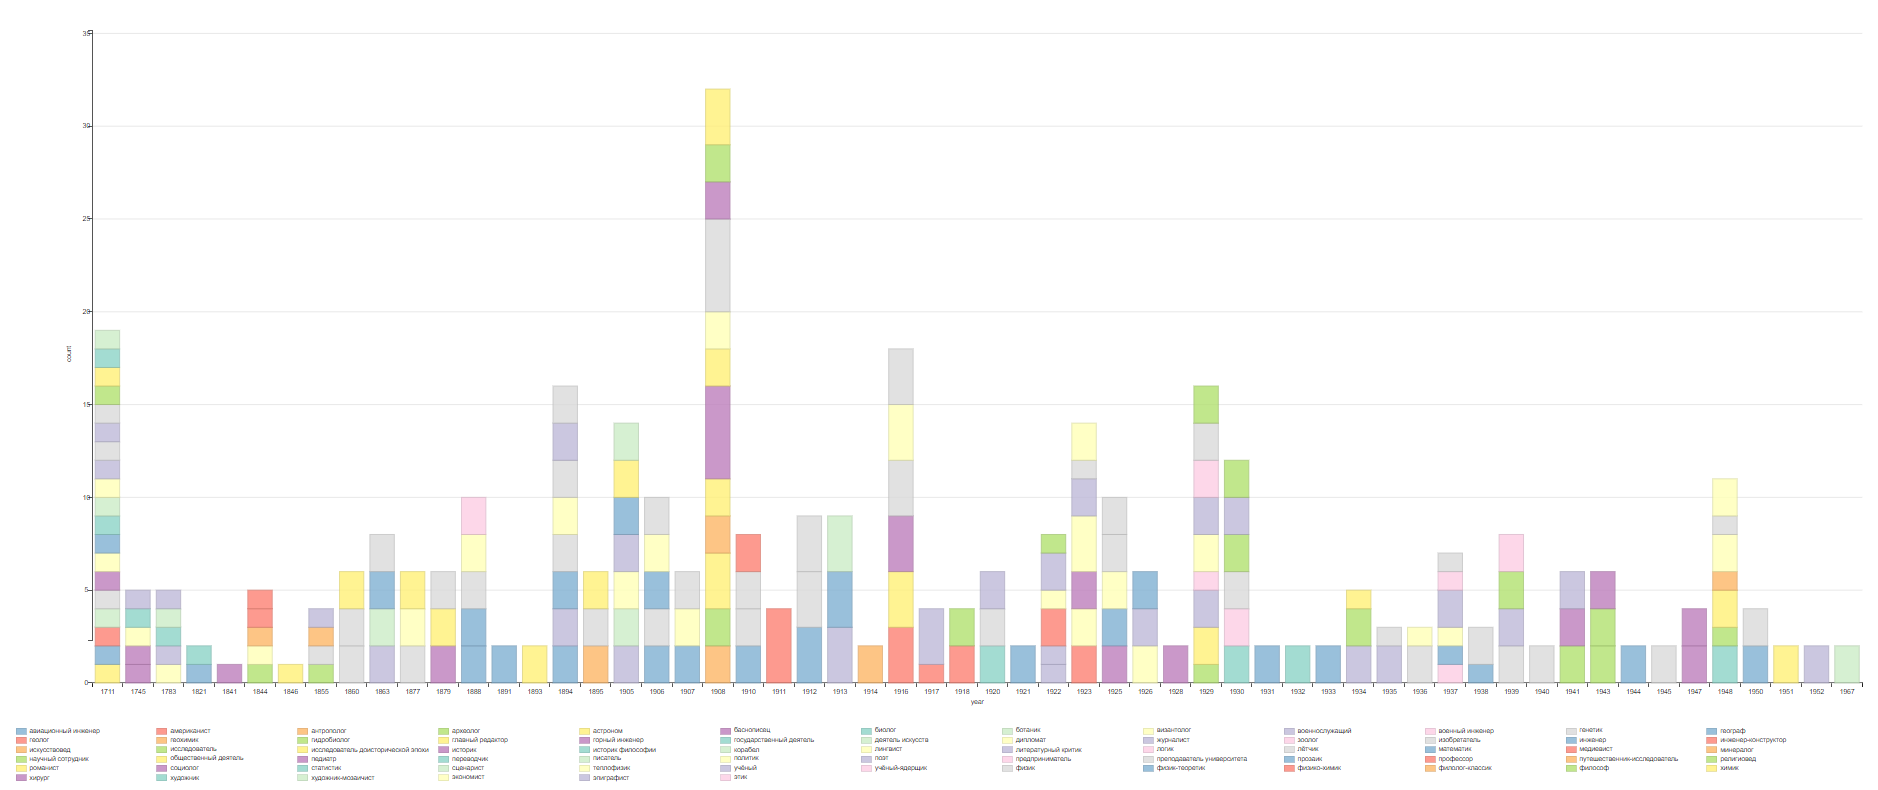
\includegraphics[width=1\linewidth]{./chapter/human_settlement/RussianScientistBurnVillage.png}}
	\label{fig:human-settlement-5}
	\caption[Диаграмма количества ученых по родам деятельности родившихся в сельских полесениях.]{Диаграмма количества ученых по родам деятельности родившихся в сельских полесениях. Ссылка на SPARQL-запрос: \href{}{Длинная ссылка}.}%
\end{figure*} 

\begin{figure*}
    \setlength{\fboxsep}{0pt}%
    \setlength{\fboxrule}{1pt}%
    \fcolorbox{gray}{gray}{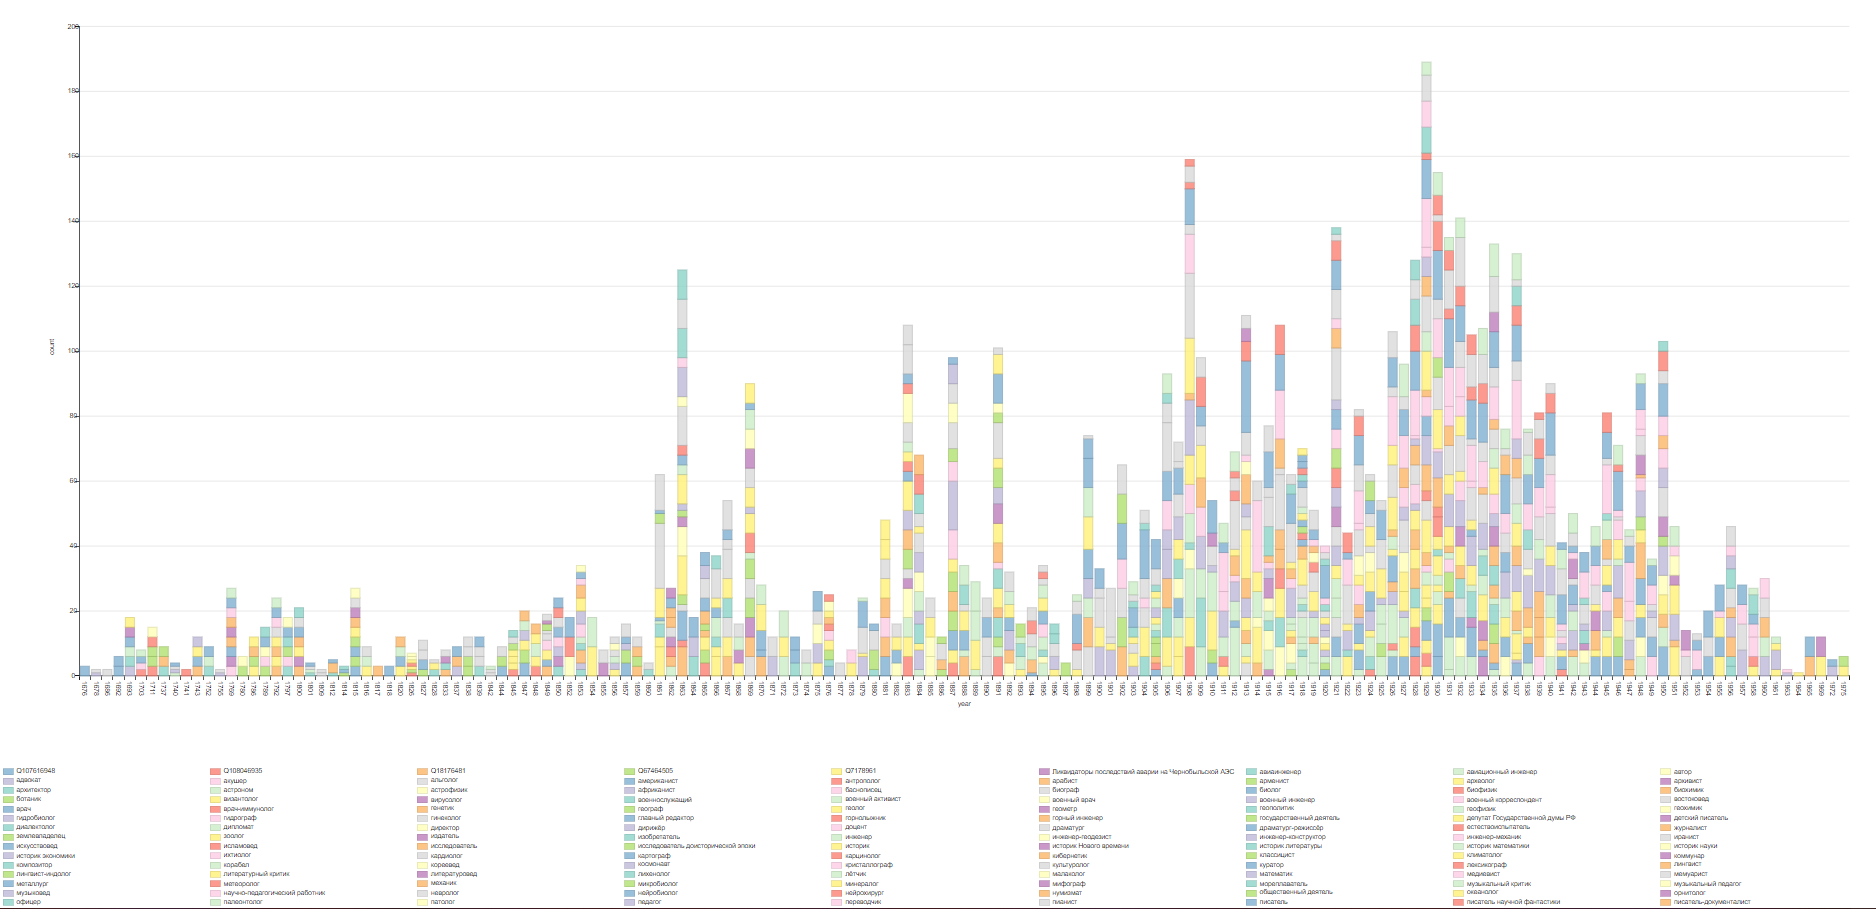
\includegraphics[width=1\linewidth]{./chapter/human_settlement/RussianScientistBurnTown.png}}
	\label{fig:human-settlement-6}
	\caption[Диаграмма количества ученых по родам деятельности родившихся в городских полесениях.]{Диаграмма количества ученых по родам деятельности родившихся в городских полесениях. Ссылка на SPARQL-запрос: \href{}{Длинная ссылка}}%
\end{figure*} 
